% Created 2018-06-21 Thu 12:30
\documentclass[8pt]{beamer}
\usetheme{Montpellier}
\usecolortheme{dove}

\usepackage[sc,osf]{mathpazo}   % With old-style figures and real smallcaps.
\linespread{1.025}              % Palatino leads a little more leading
% Euler for math and numbers
\usepackage[euler-digits,small]{eulervm}
%\documentclass[10pt]{llncs}
%\usepackage{llncsdoc}
\usepackage{changepage}
\usepackage{minted}
\usepackage[utf8]{inputenc}
\usepackage[T1]{fontenc}
\usepackage{fixltx2e}
\usepackage{graphicx}
\usepackage{longtable}
\usepackage{float}
\usepackage{wrapfig}
\usepackage{rotating}
\usepackage[normalem]{ulem}
\usepackage{amsmath}
\usepackage{textcomp}
\usepackage{marvosym}
\usepackage{wasysym}
\usepackage{amssymb}
\usepackage{hyperref}
\usepackage{polynom}
\renewcommand{\mod}[1]{\left( \texttt{mod}~#1 \right)}
\newcommand{\N}{\mathbb N}
\newcommand{\Z}{\mathbb Z}
\newcommand{\Q}{\mathbb Q}
\newcommand{\C}{\mathbb C}
\newcommand{\nt}{\Rightarrow}
\newcommand{\cat}[1]{\mathsf{#1}}
\newcommand{\cSet}{\cat{Set}}
\newcommand{\cCone}{\cat{Cone}}
\newcommand{\Hom}{\ensuremath{\operatorname{Hom}}}
\tolerance=1000
\usetheme{Antibes}
\author{Siddharth Bhat}
\date{Sun 20, June 2021}
\institute{\texttt{\#\#harmless} Category Theory in Context}
\title{Limits and Colimits as universal cones}
\hypersetup{
  pdfkeywords={},
  pdfsubject={},
  pdfcreator={Emacs 24.5.1 (Org mode 8.2.10)}}
\begin{document}

\maketitle

\begin{frame}[fragile]{Building objects from other ones}
    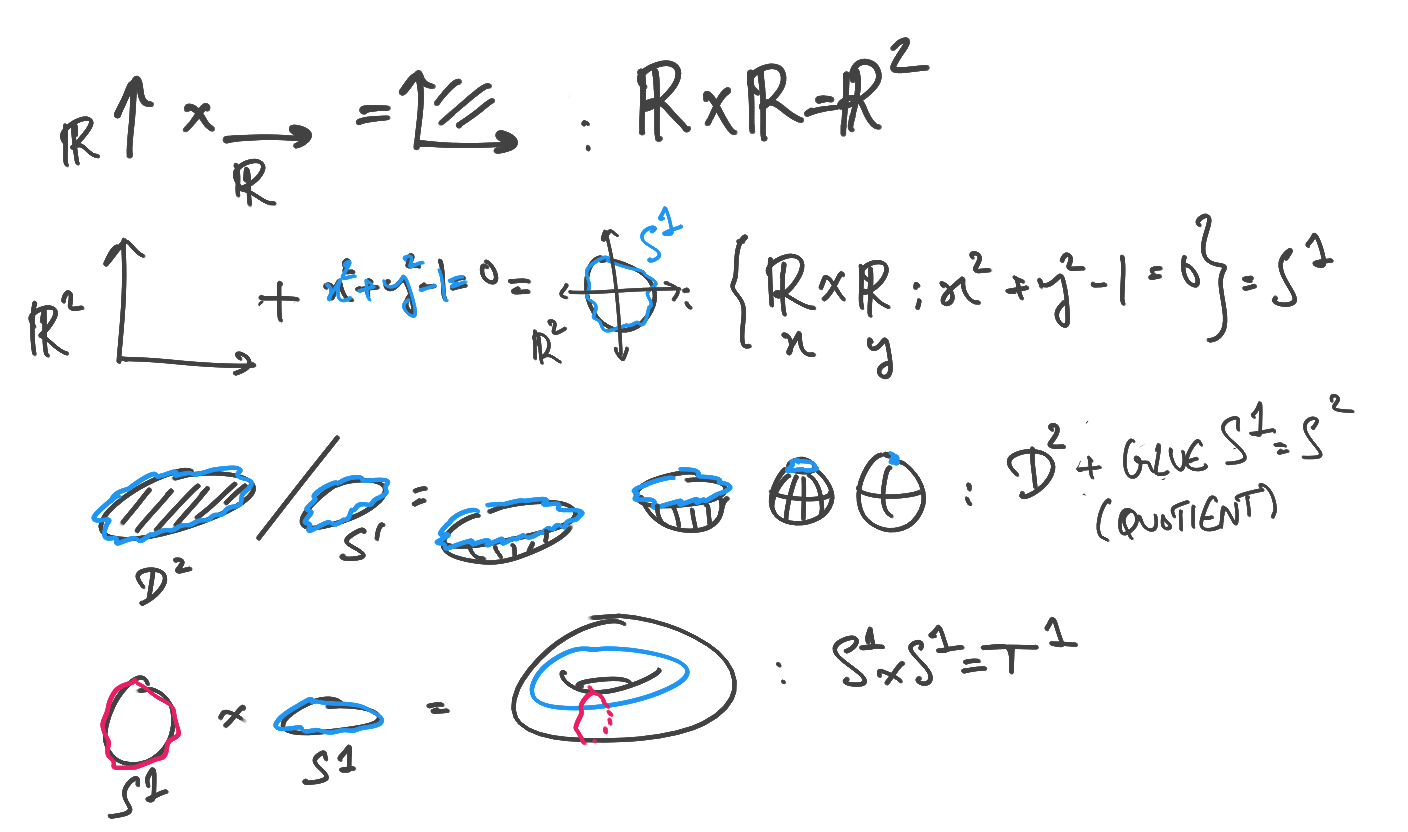
\includegraphics[width=\textwidth]{./examples-of-limits.png}
\end{frame}

\begin{frame}[fragile]{Cone over a diagram (Picture)}
    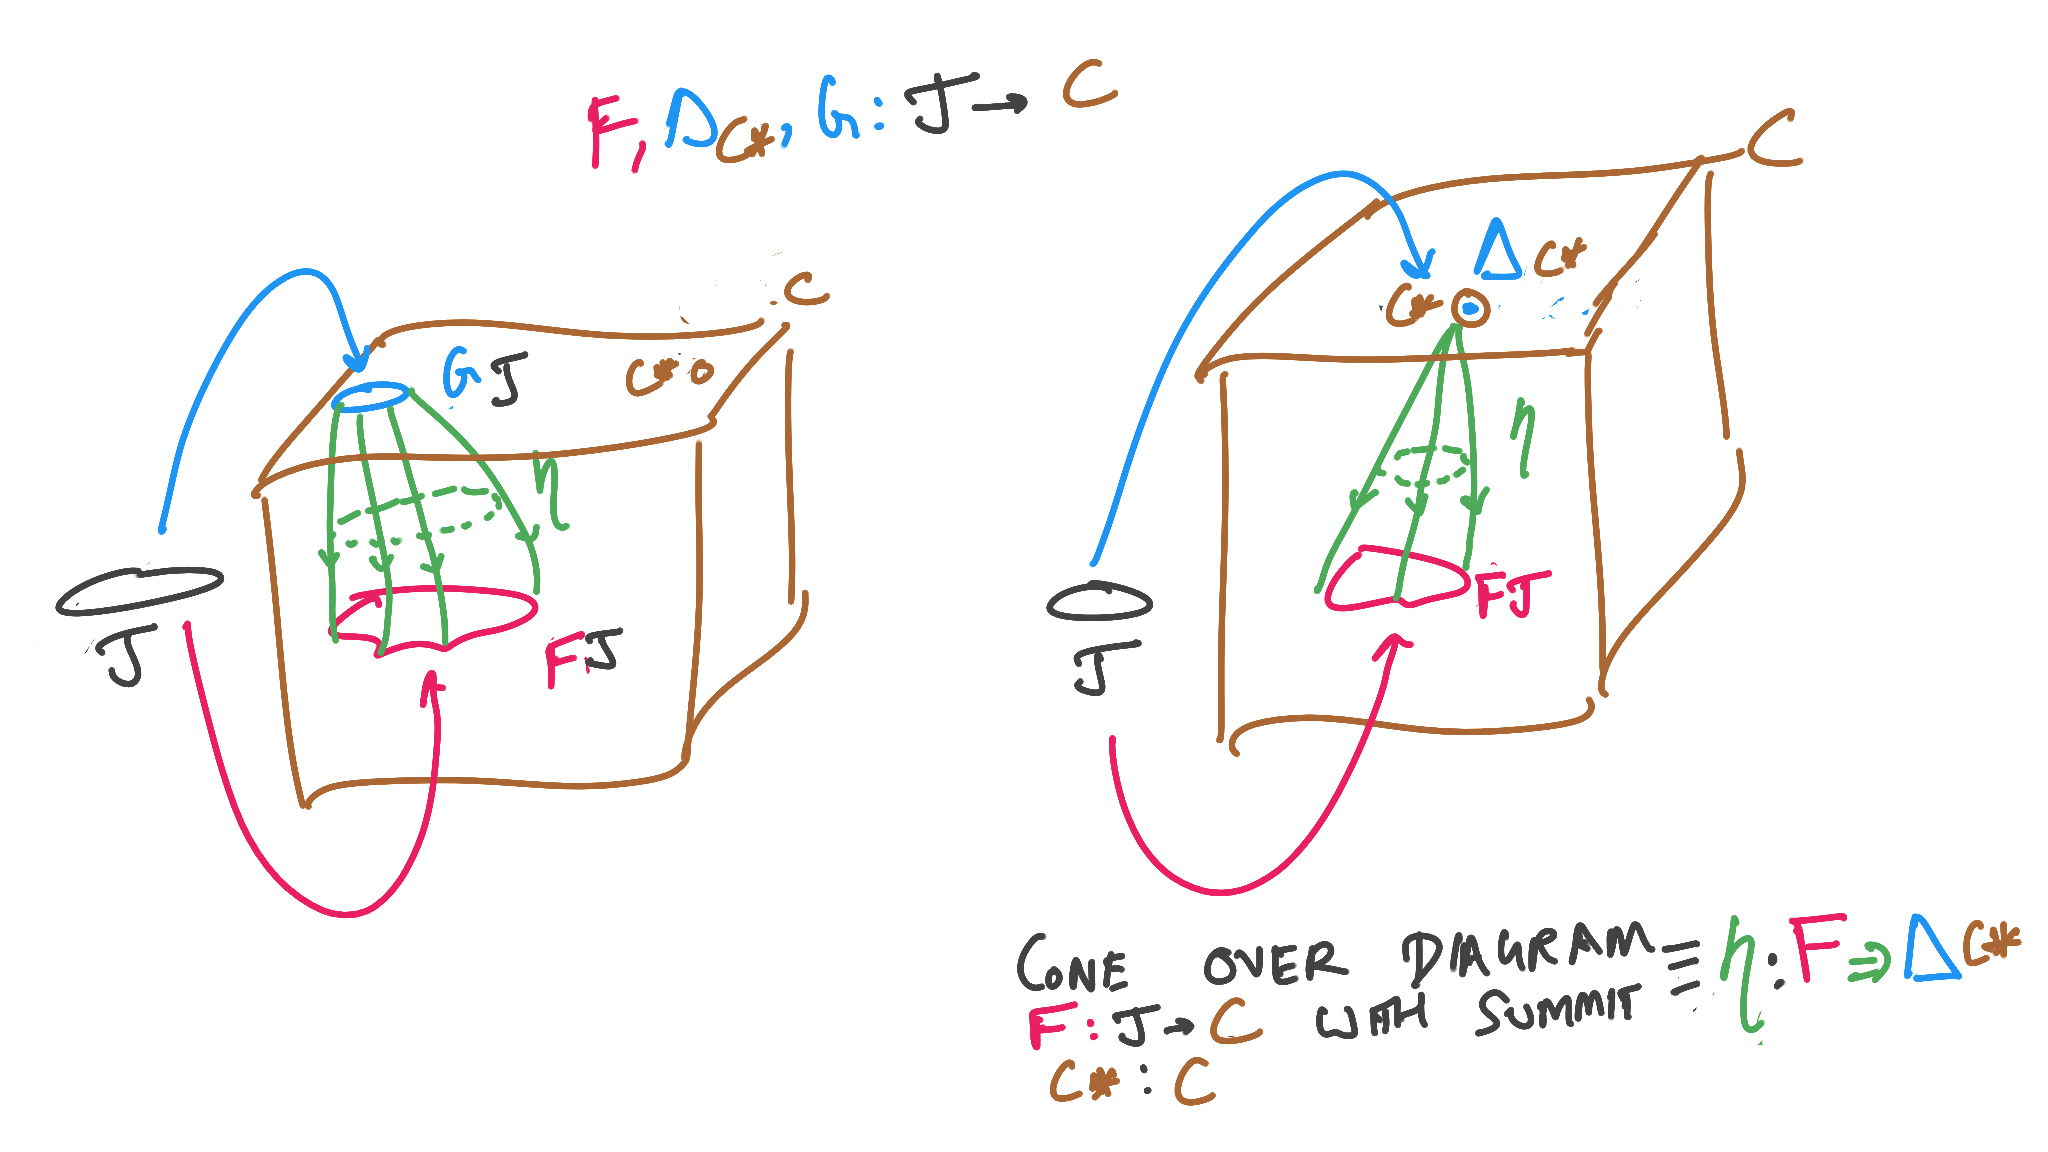
\includegraphics[width=\textwidth]{./cone.png}
\end{frame}


\begin{frame}[fragile]{Cone over a diagram (formally)}
    \begin{columns}[T] % align columns
        \begin{column}{.48\textwidth}
            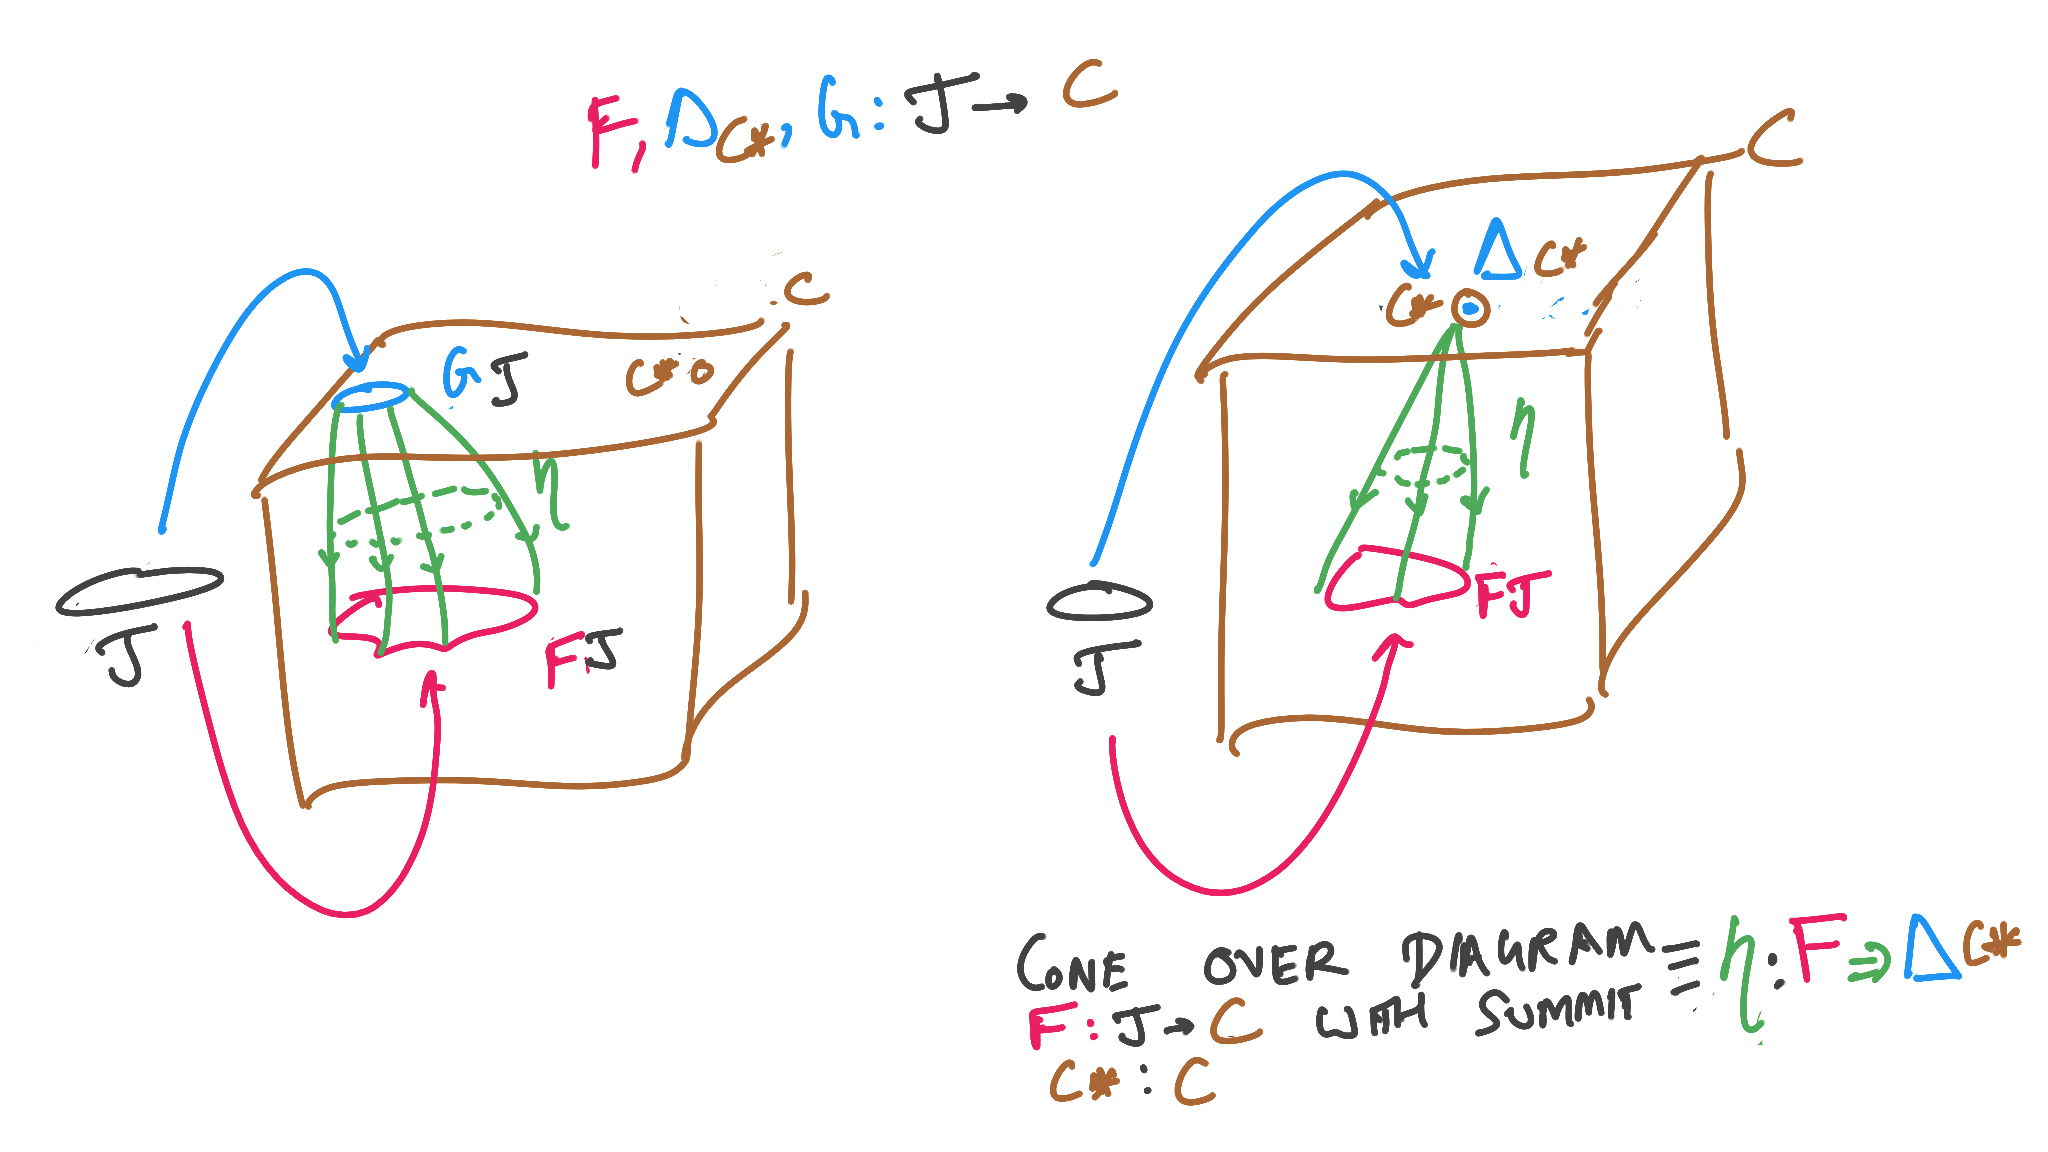
\includegraphics[width=\textwidth]{./cone.png}
        \end{column}

    \begin{column}{.48\textwidth}
    \begin{itemize}
        \item Given: (1) a diagram category $J$, (2) a target category $C$, (3) a functor $F: J \to C$, (4)
              a choice of apex $c_* \in C$. \pause
        \item The cone is: A natural transformation $\eta$ between the constant functor $\Delta_{c_*}: J \to C$ 
            (defined by the eqn $\Delta_{c_*}(\_) \equiv c_*$) and the given $F: J \to C$. \pause
        \item At each component, we have:
            \begin{align*}
                &\eta: \Delta_{c_*} \nt F \\
                &\eta_j: \Delta_{c_*}(j) \to F(j) \\
                &\eta_j: c_* \to F(j) \\
            \end{align*}
    \end{itemize}
    \end{column}
    \end{columns}
\end{frame}

\begin{frame}[fragile]{Cone over a diagram (\texttt{DependentHaskell})}
    % \begin{adjustwidth}{-2em}{-2em}
    \begin{columns}[T] % align columns
        \begin{column}{.48\textwidth}
            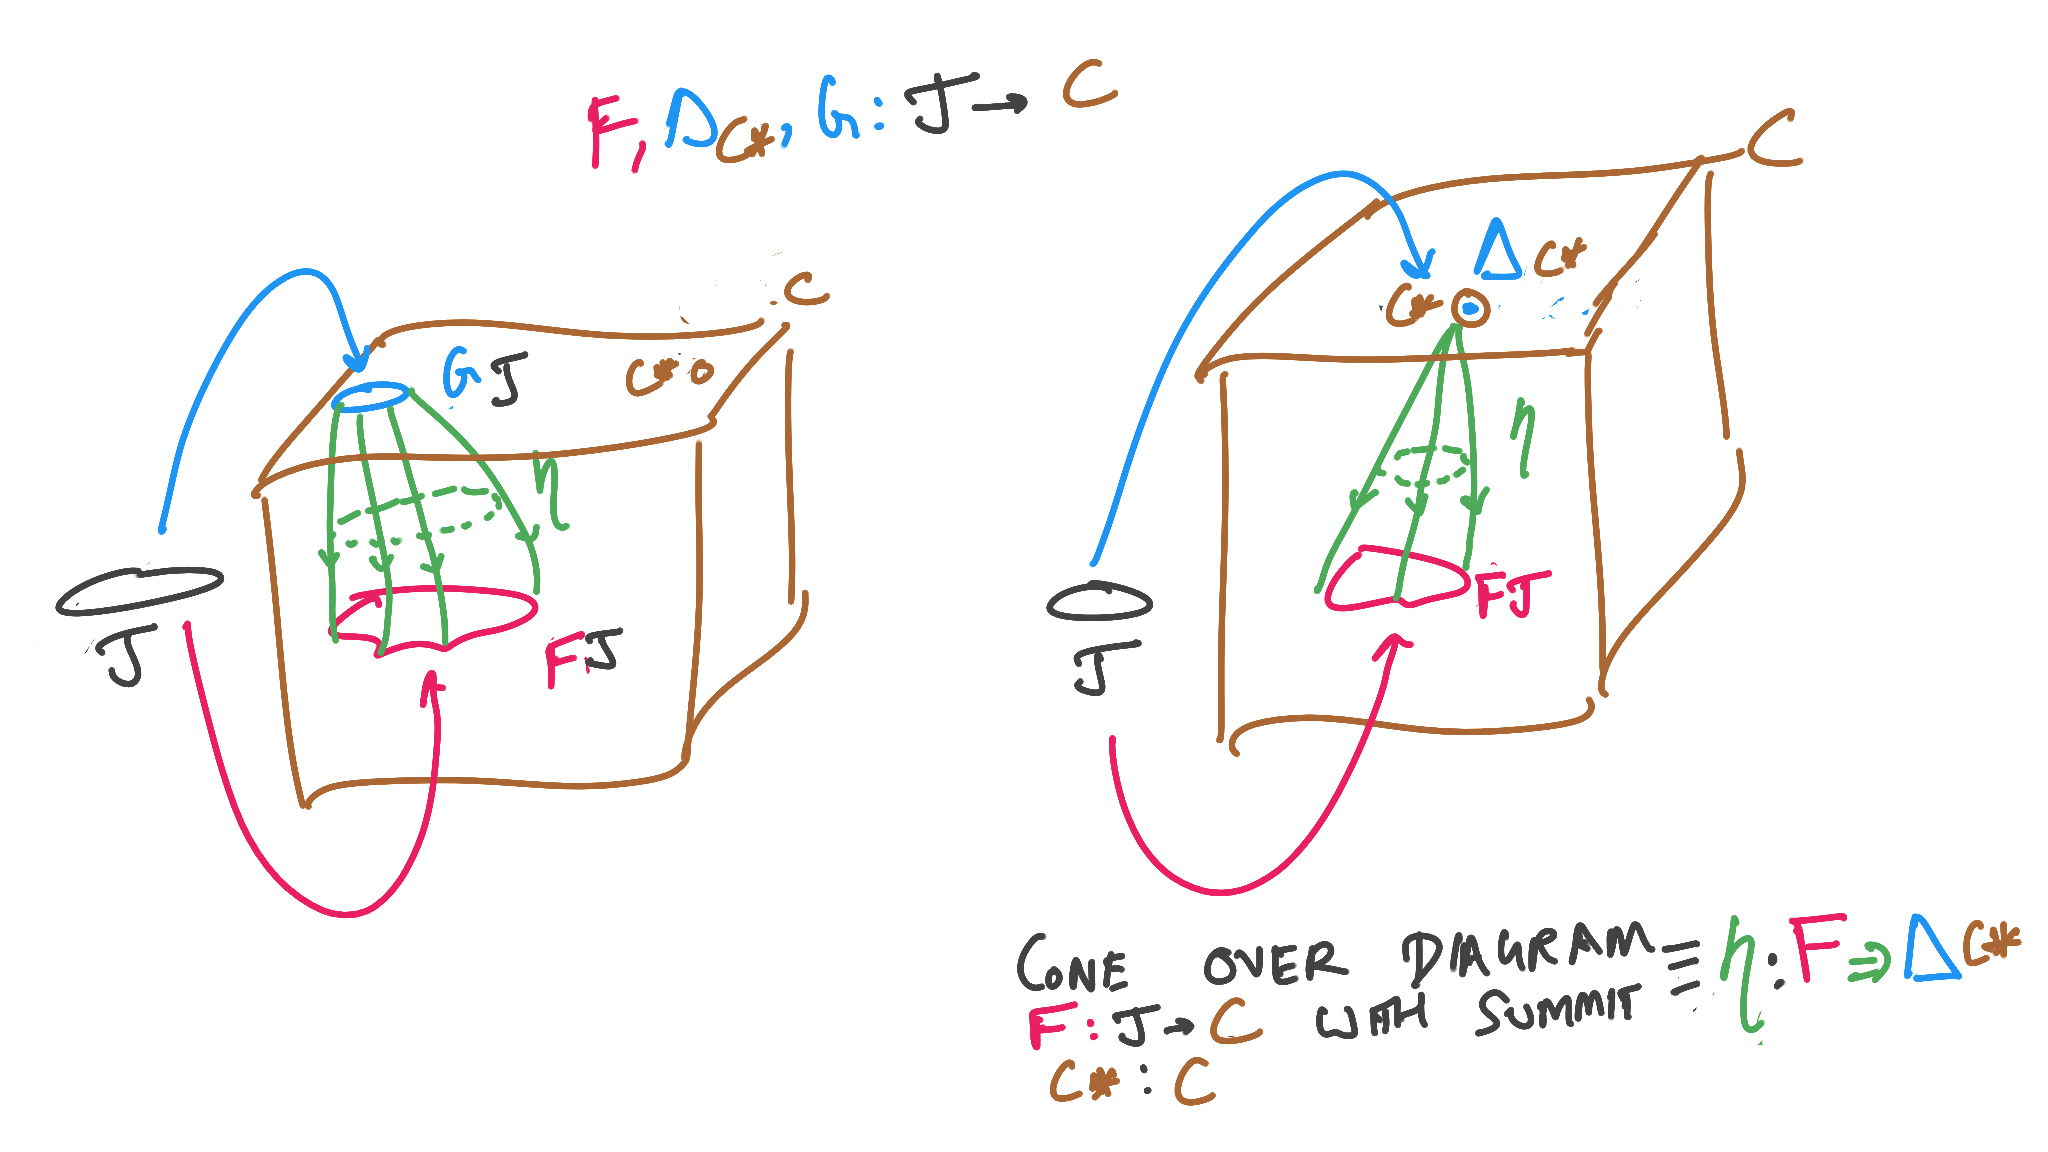
\includegraphics[width=\textwidth]{./cone.png}
    {\footnotesize
    \begin{itemize}
        \item Given: (1) a diagram category $J$, (2) a target category $C$, (3) a functor $F: J \to C$, (4)
              a choice of apex $c_* \in C$. 
        \item The cone is: A natural transformation $\eta$ between the constant functor $\Delta_{c_*}: J \to C$ 
            (defined by the eqn $\Delta_{c_*}(\_) \equiv c_*$) and the given $F: J \to C$. 
        \item At each component, we have:
            \begin{align*}
                &\eta: \Delta_{c_*} \nt F \\
                &\eta_j: \Delta_{c_*}(j) \to F(j) \\
                &\eta_j: c_* \to F(j) \\
            \end{align*}
    \end{itemize}
    }
    \end{column}

    \begin{column}{.6\textwidth}
        {\tiny
        \begin{minted}{hs}
            ConstFunctor (J :: Category) (C :: Category) (c :: C) = 
              Functor J C
                (\j -> c) -- action on objects
                (\a -> id c)  -- action on arrows

            Cone (J :: Category) (C :: Category) 
                 (c :: C) (F :: Functor J C)  = 
                   NaturalTransformation (ConstFunctor C c) F
        \end{minted}
        }
    \end{column}
    \end{columns}
\end{frame}

\begin{frame}{Example Cone 1}
    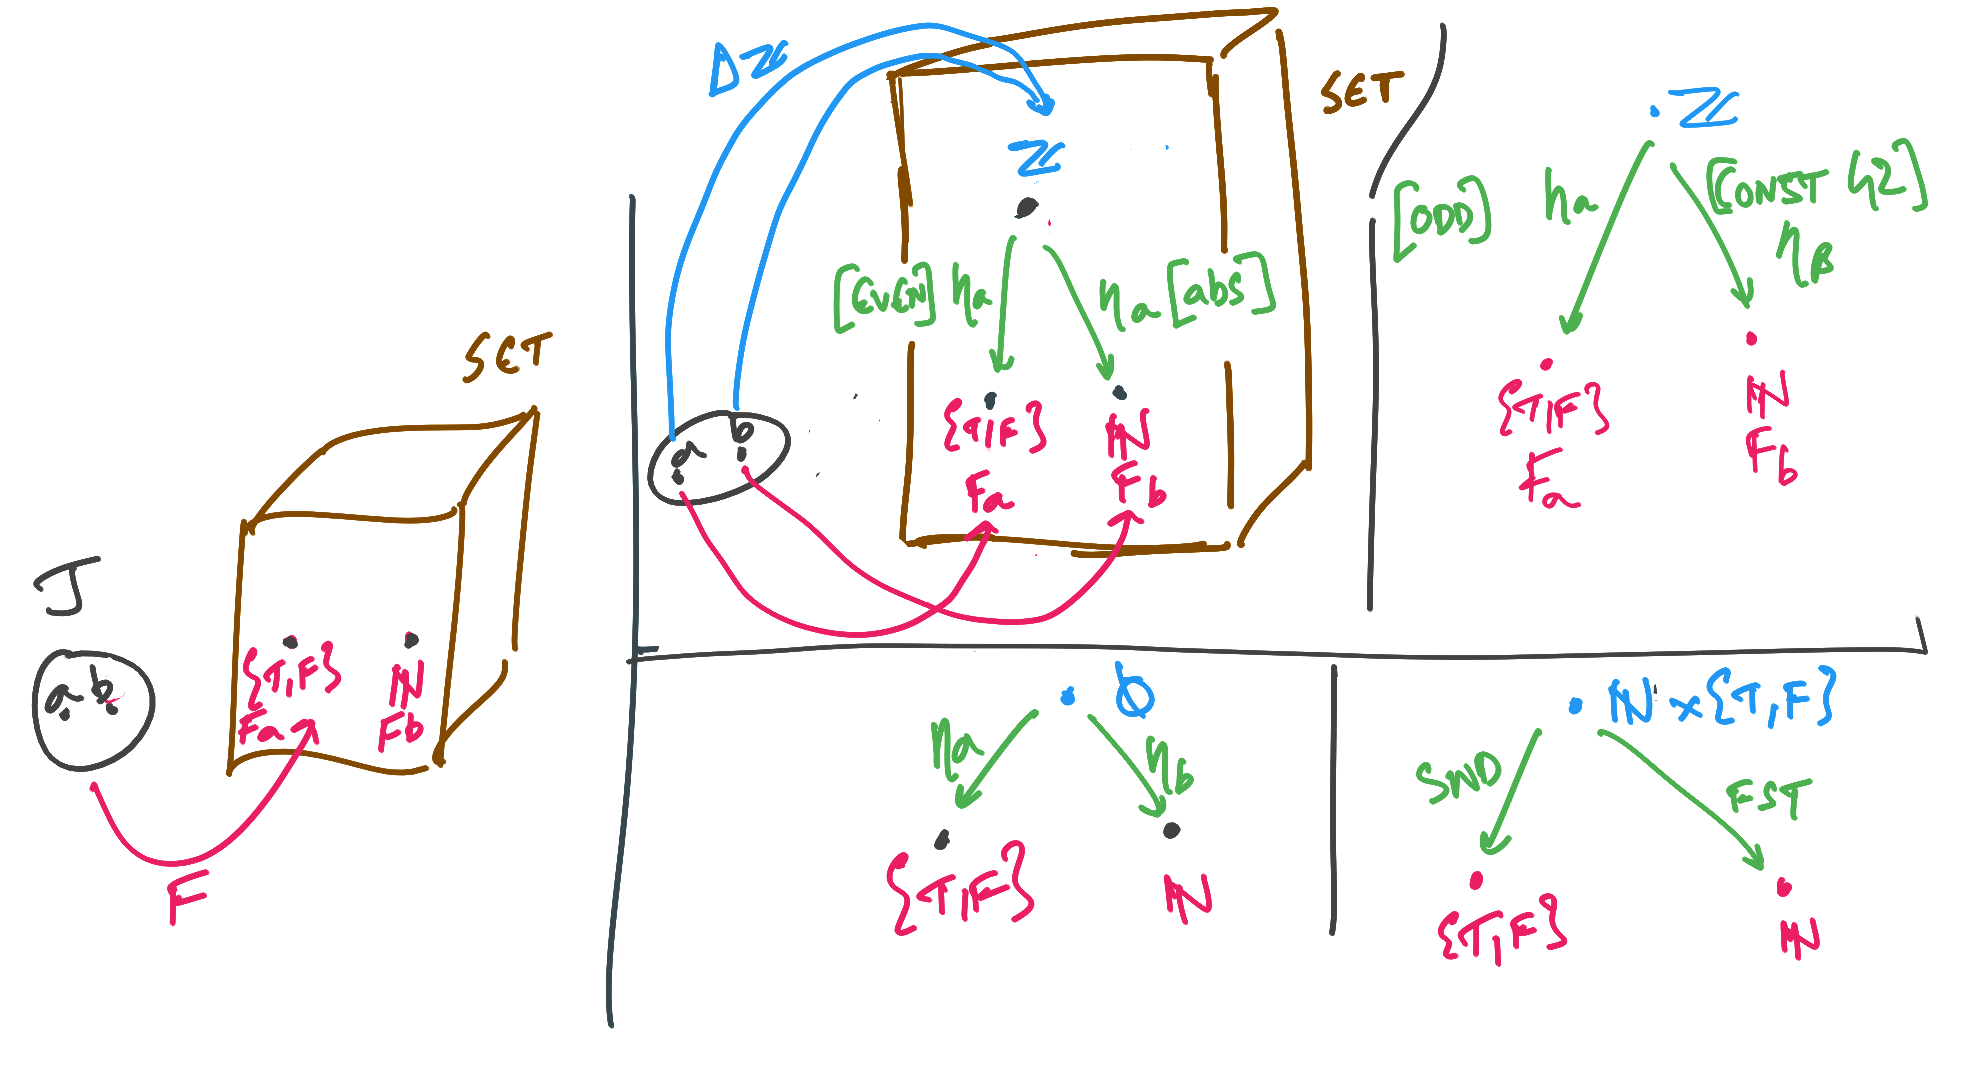
\includegraphics[width=\textwidth]{./cones-over-discrete.png}
\end{frame}

\begin{frame}{Example Cone 2}
    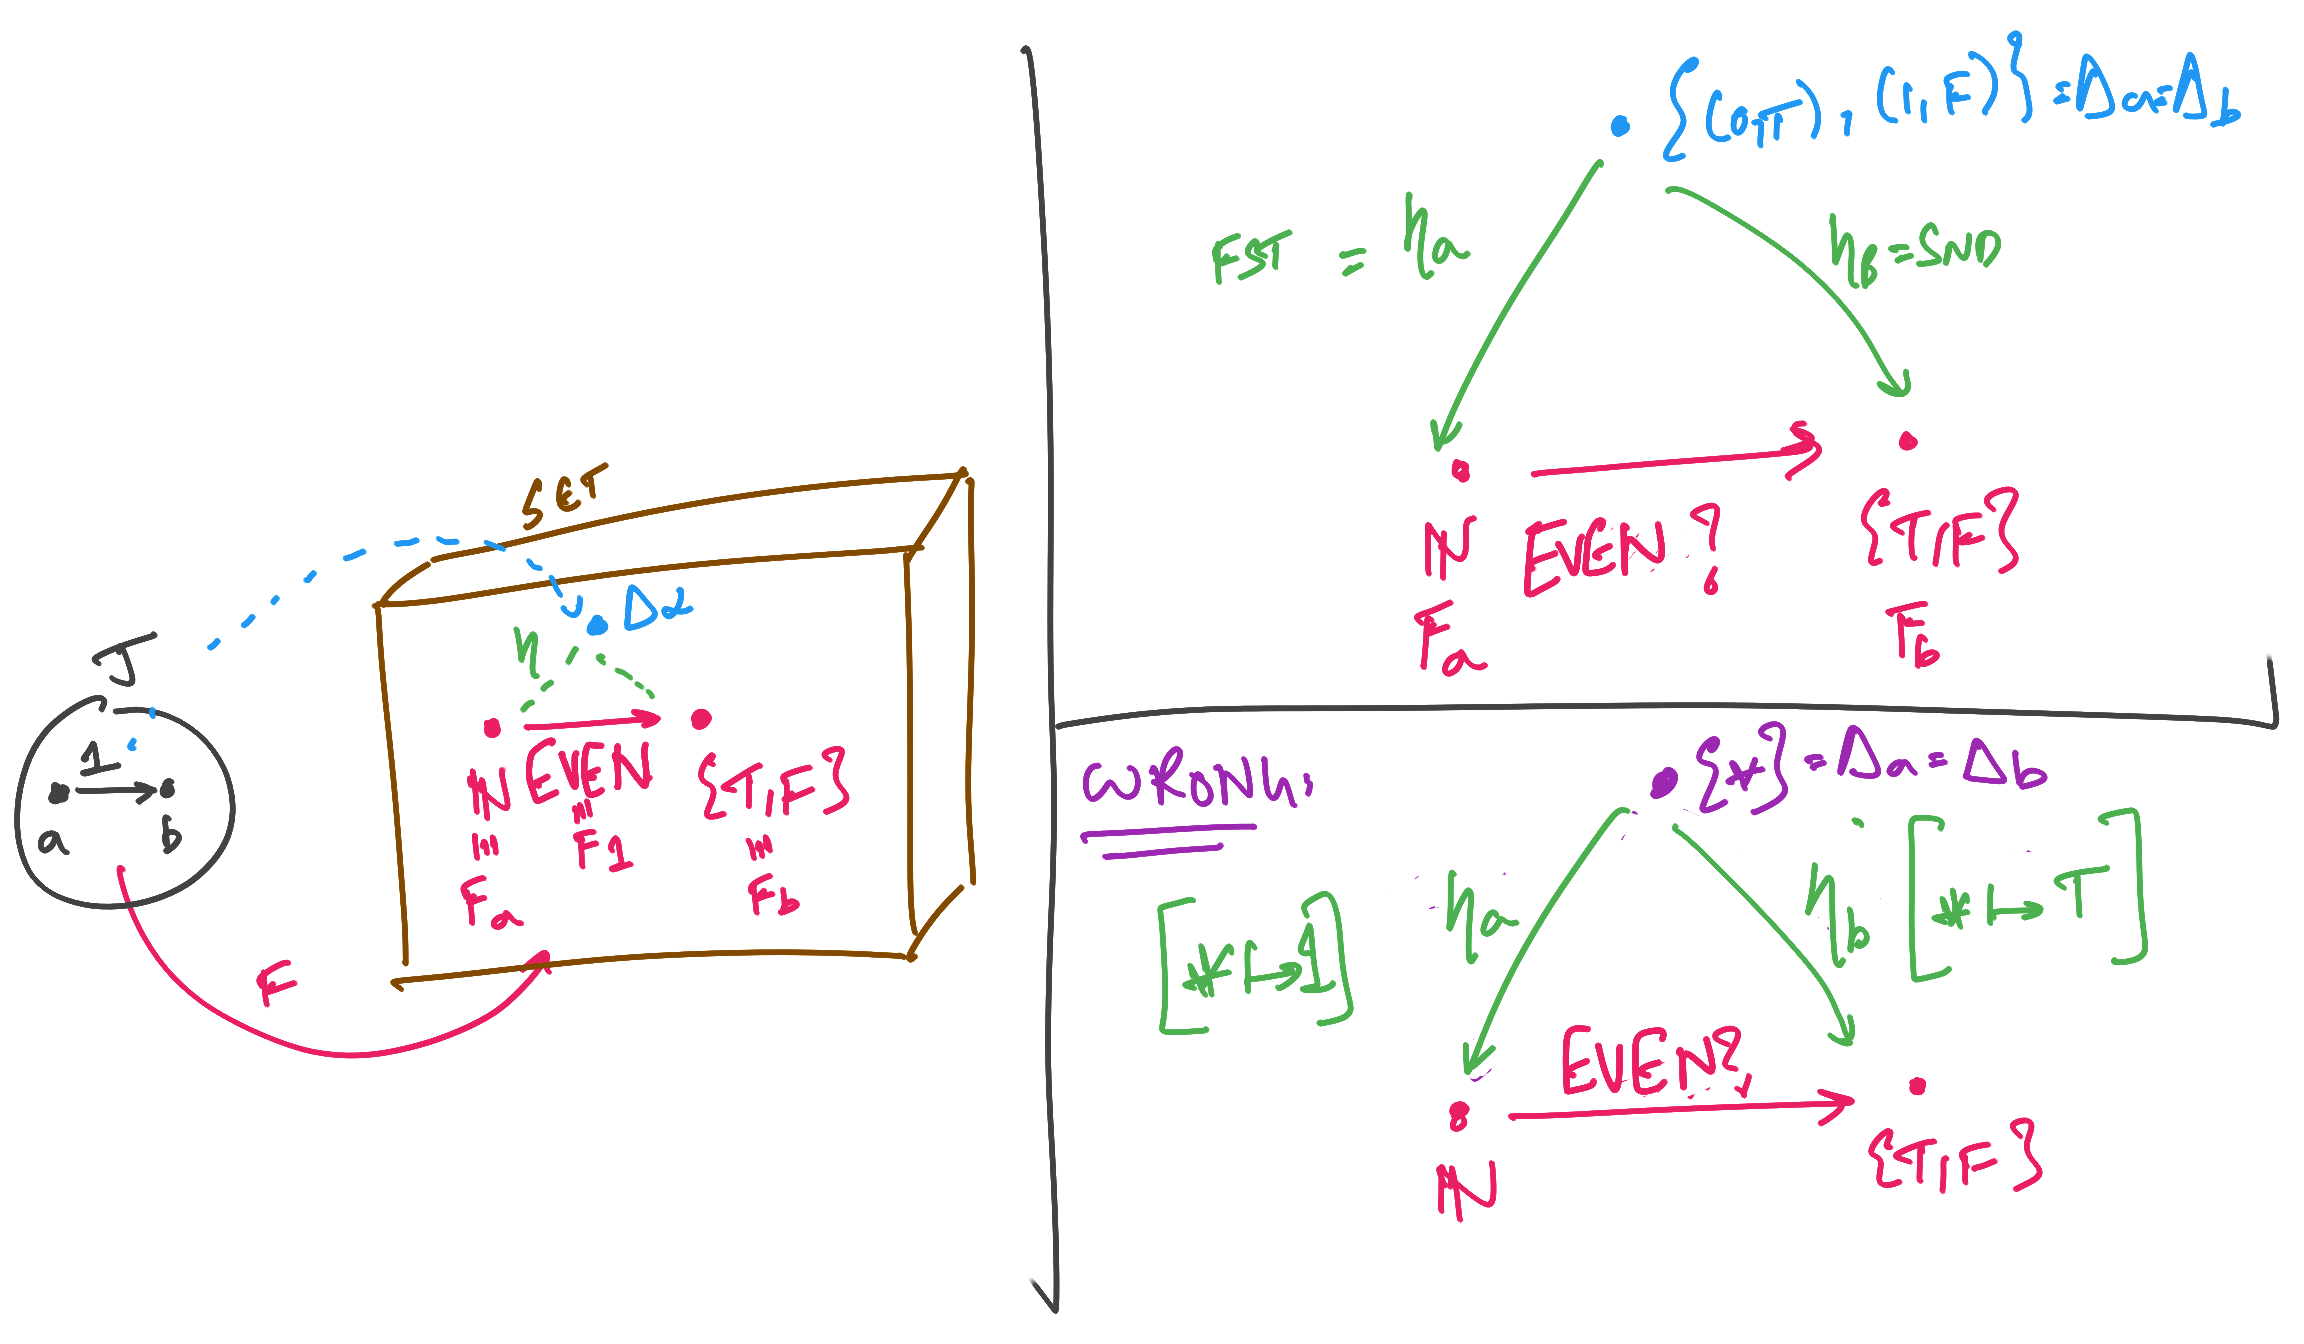
\includegraphics[width=\textwidth]{./cones-over-single-arrow.png}
\end{frame}

\begin{frame}{Definition of a Limit 1}
    \begin{columns}[T] % align columns
        \begin{column}{.48\textwidth}
            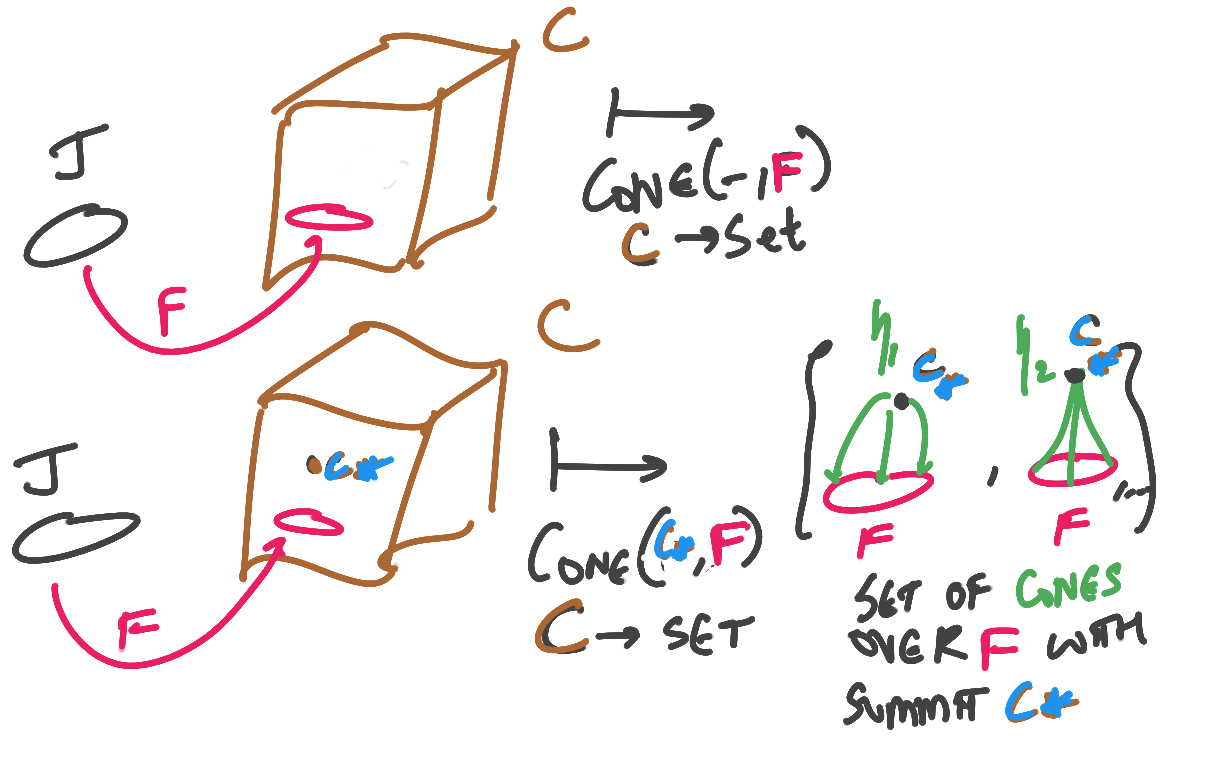
\includegraphics[width=\textwidth]{./cone-functor.png}
            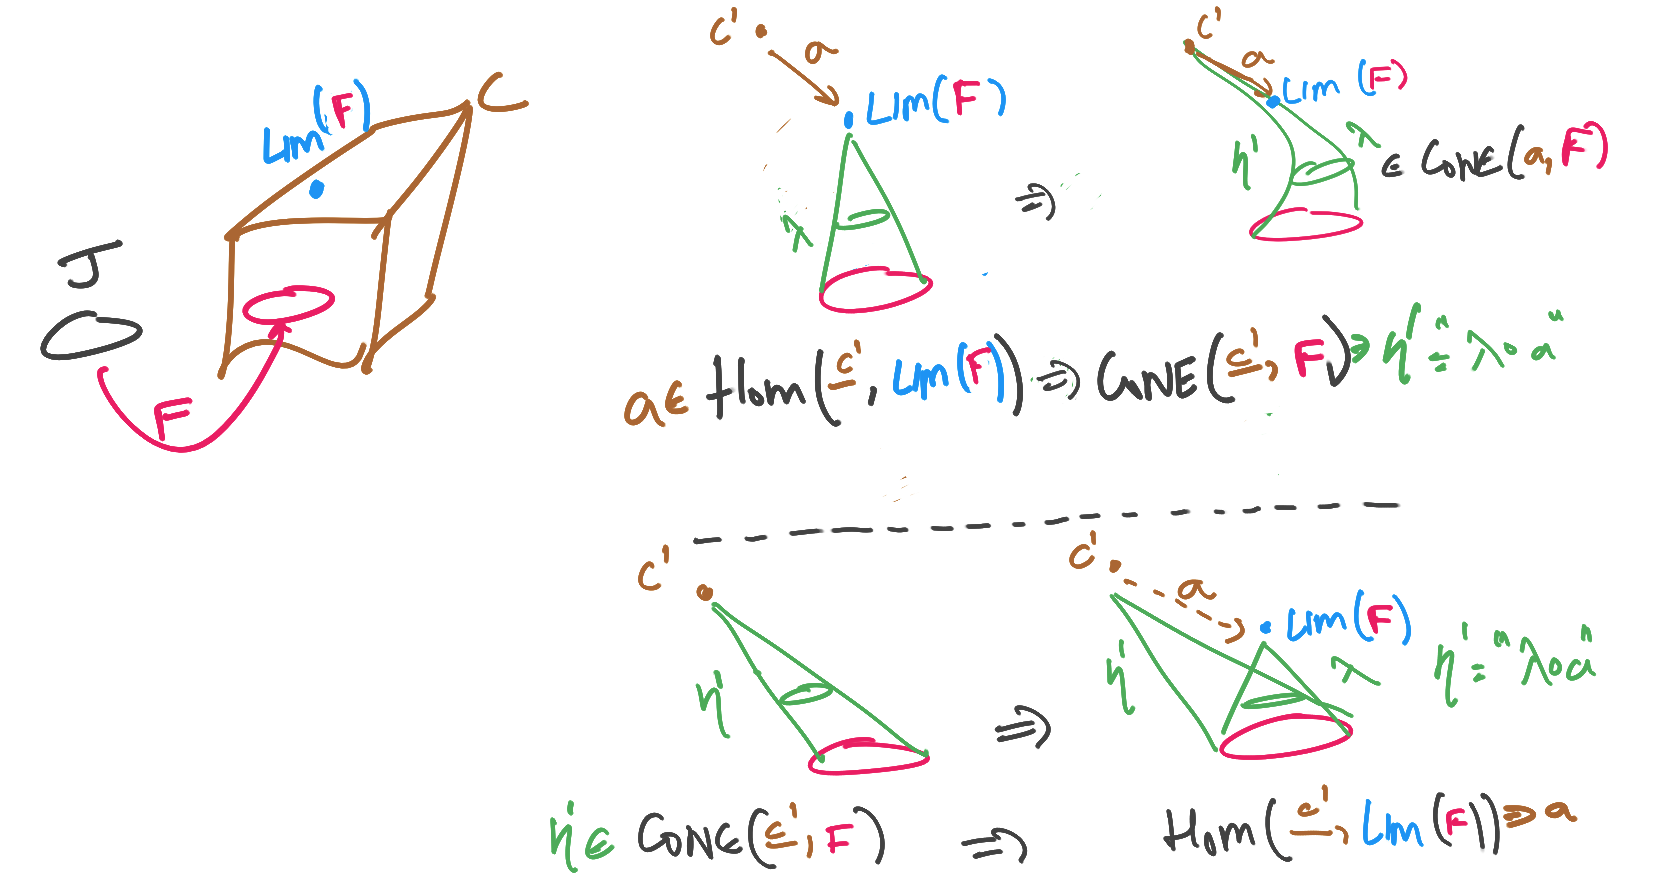
\includegraphics[width=\textwidth]{./natural-iso-limit-cone.png}
        \end{column}
        \begin{column}{.6\textwidth}
     \begin{itemize}
         \item For any diagram $F: J \to C$, there is a functor: $\cCone(-, F): C \to \cSet$ which sends
             a given object $c_* \in C$  to the set of cones over $F$ with summit $c_*$. \pause
        \item A limit is a representation of $\cCone(-, F)$. \pause
        \item So we have an object $\lim F$ whose Hom functor represents $\cCone(-, F)$.
              This is given by $\eta: \Hom_C(-, \lim F) \simeq \cCone(-, F)$. \pause
        \item By Yoneda, such a natural transformation is determined entirely by an element of
            $\cCone(-, F)(\lim F)$, or $\cCone(\lim F, F)$. \pause
        \item Call this (universal) element $\lambda \in \cCone(\lim F, F)$. This is a natural transformation
            $\lambda : \Delta_{\lim F} \nt F$. \pause \footnote{Riehl writes $\lambda: \lim F \nt F$ which does not type-check for me.}
     \end{itemize}
    \end{column}
    \end{columns}
\end{frame}

\begin{frame}{Definition of a Limit 1: Natural Iso}
    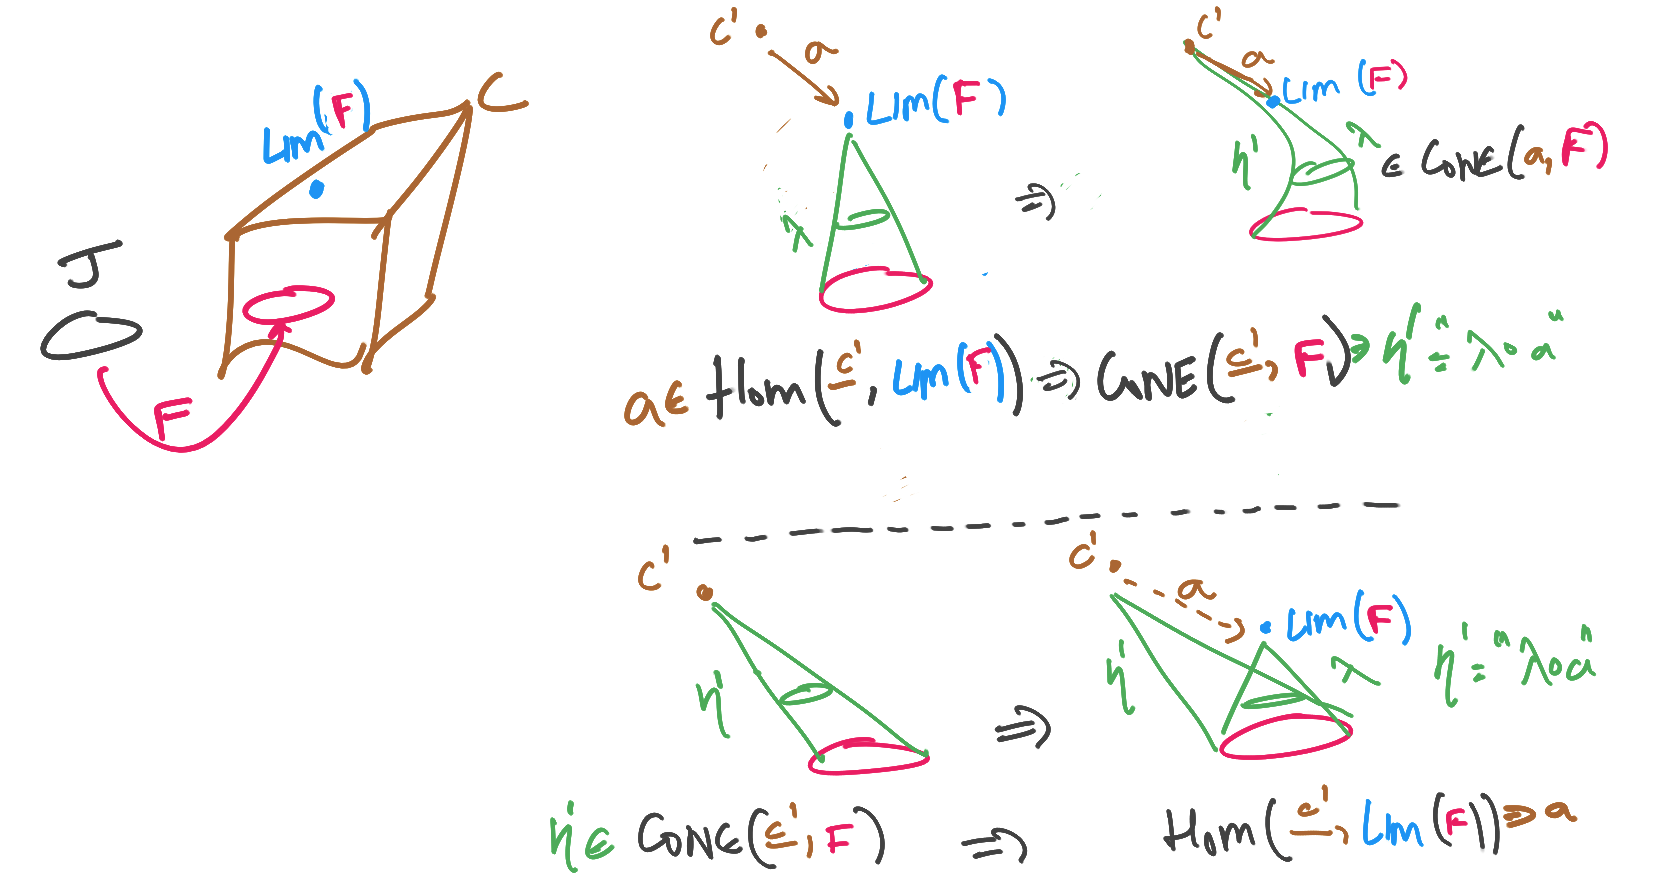
\includegraphics[width=\textwidth]{./natural-iso-limit-cone.png}
    {\footnotesize
    \begin{itemize}
    \item An object $\lim F$ such that $\eta: \Hom_C(-, \lim F) \simeq \cCone(-, F)$. 
    \item By Yoneda, $\eta$ is determined entirely by an element of $\cCone(\lim F, F)$. 
    \item This Universal element is $\lambda \in \cCone(\lim F, F)$. Ie, a natural transformation $\lambda : \Delta_{\lim F} \nt F$. 
     \end{itemize}
    }
\end{frame}

\begin{frame}{Definition of a Limit 2: Terminal in category of elements}
    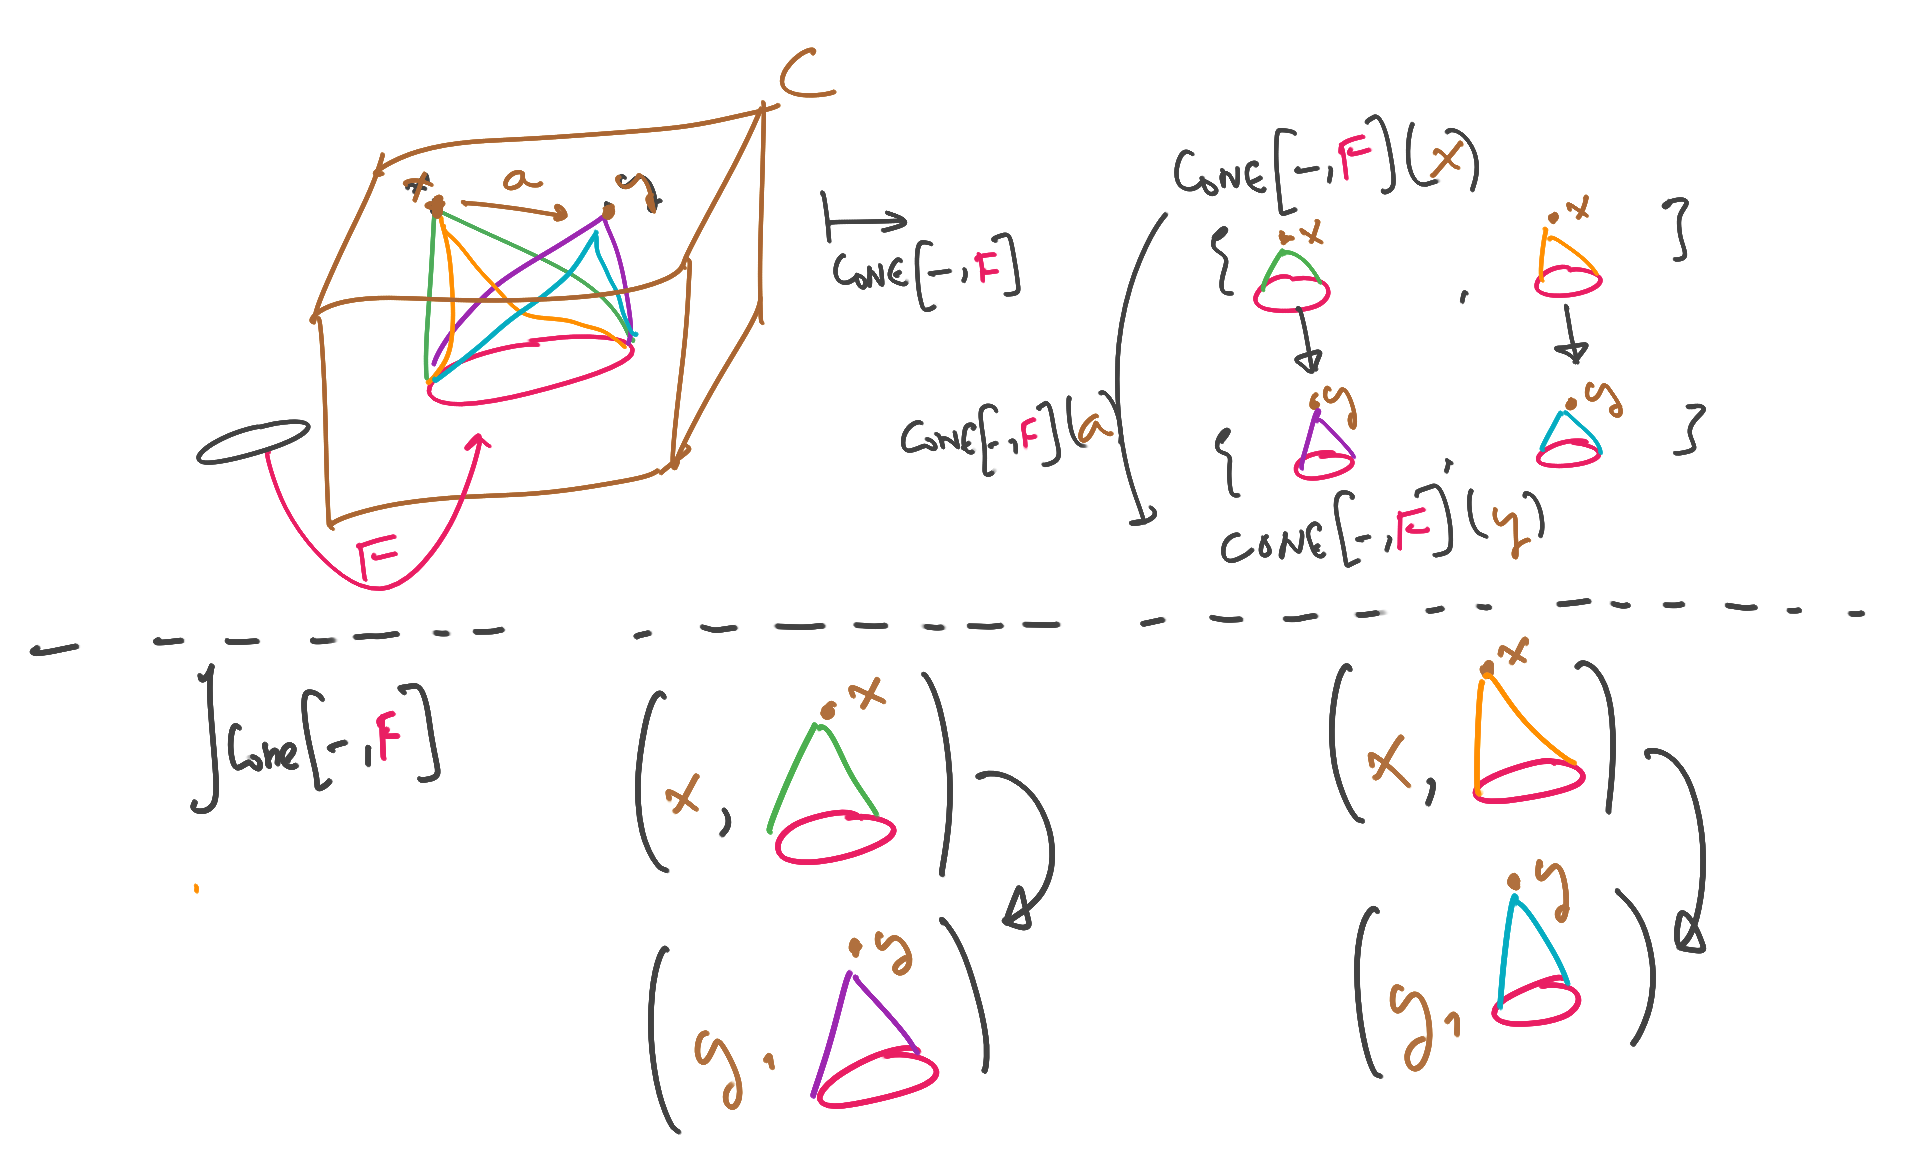
\includegraphics[width=0.8\textwidth]{./category-of-elements-description.png}
    {\footnotesize
    \begin{itemize}
        \item category of elements of $\cCone(-, F): C \to \cSet$ for a given functor $F: J \to C$?
        \item object: $(x \in C, \eta_x) \in \cCone(x, F) \in cSet$. So, a pair of a summit $x$
            and a cone with summit $x$ and base $F: J \to C$.
        \item Objects of the category of elements: cones with different summits.
        \item Arrows in the category of elements: Arrows $ x \xrightarrow{a} y$
            in $C$ such that for elements $(x, \eta_x)$ and $(y, \eta_y)$, the
            functor $\cCone(-, F)$ obeys $\cCone(-, F)(a)(\eta_x) = \eta_y$.
            \footnote{I just realised that the morphisms of this cone functor
            have not been defined by Riehl!}
    \end{itemize} }
\end{frame}

\begin{frame}{Definition of a Limit 2: Terminal in category of elements}
    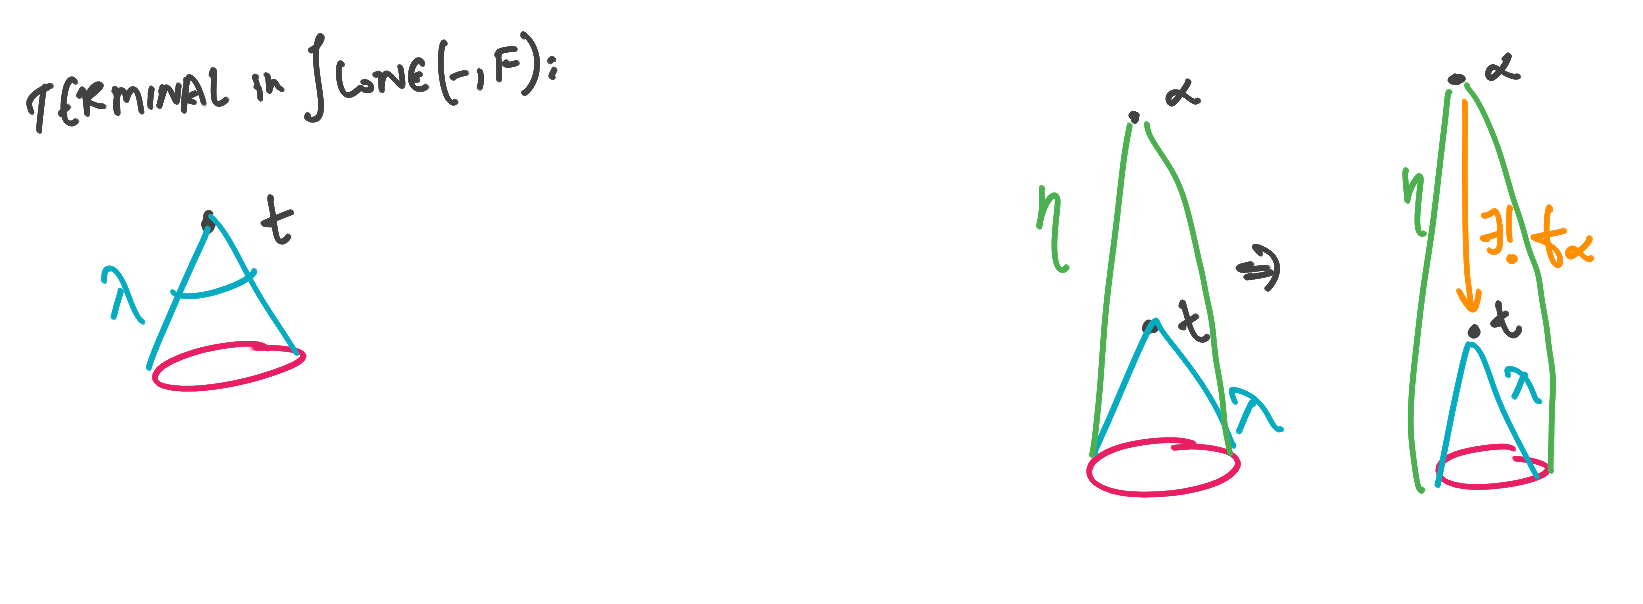
\includegraphics[width=\textwidth]{./category-of-elements-terminal.png}
    \begin{itemize}
        \item All cones $(\alpha:C, \Delta_\alpha \nt_\eta F : [J, C])$ 
            factor through the terminal cone $(t: C, \Delta_t \nt_\lambda F : [J, C]$).
    \end{itemize}
\end{frame}


\begin{frame}{Limit example 1 :(Empty diagram)}
    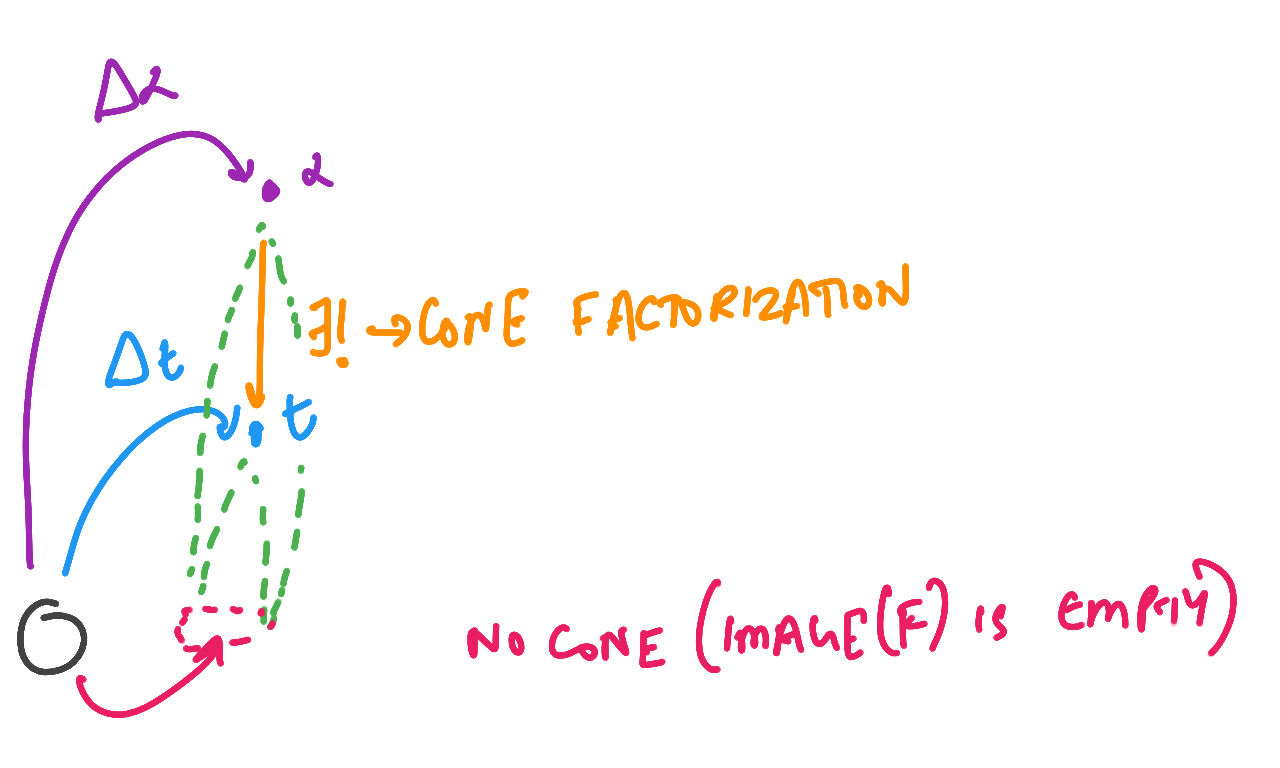
\includegraphics[width=\textwidth]{./empty-diagram-limit.png}
\end{frame}

\begin{frame}{Limit example 2 : (Discrete diagram)}
    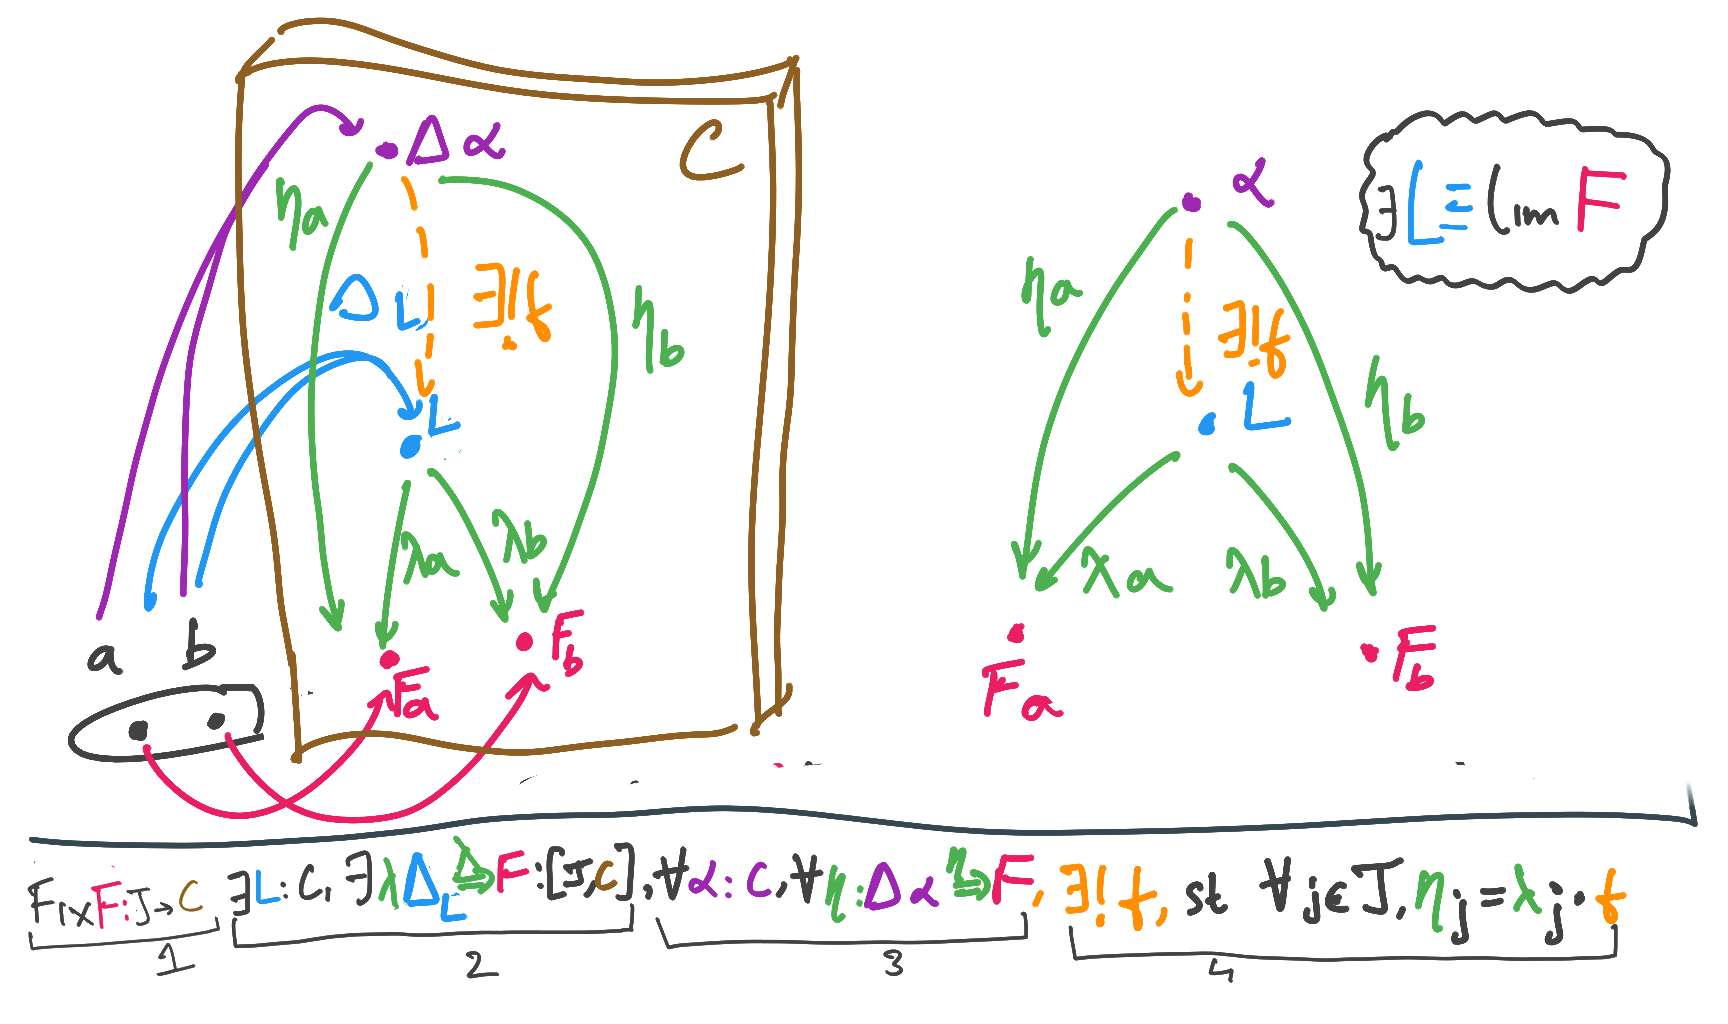
\includegraphics[width=\textwidth]{./discrete-diagram-limit.png}
\end{frame}

\end{document}
